% ----------------------------------------------------------------------------------------------------- %
% Manual da Classe UFTeX
% 
% Versão 2.1:   Março 2018
%
% Criado por:   Tiago da Silva Almeida
% Revisado por: Tiago da Silva Almeida
%               Rafael Lima de Carvalho
%               Ary Henrique Morais de Oliveira
%
% https://almeidatiago.github.io/uftex/
% ----------------------------------------------------------------------------------------------------- %

\documentclass[tcc2]{classe_uftex/uftex}
% ---- Esse comando cria o nome uftex estilizado
\newcommand\uftex{UF\TeX}

\usepackage{lipsum}
\usepackage{tikz}
\usepackage[siunitx]{circuitikz}
\usetikzlibrary{arrows}

\usepackage[alf,abnt-emphasize=bf]{abntex2cite}
\renewcommand{\backrefpagesname}{}
\renewcommand{\backref}{}
\renewcommand*{\backrefalt}[4]{}
% ----  Esse comandos são necessário no pré-ambulo para a impressão da lista de lista abreviatuas e de símbolos
\makelosymbols
\makeloabbreviations
% ---- Início do documento
\begin{document}
  % ---- Descrição do título do trabalho 
  \title{Explorando Desempenho e Otimização em Algoritmos de Descoberta de Redes de Petri para Análise de Processos}
  % ---- Nome do autor ou autores do trabalho
  \author{Lucas}{Dias Barreto}
  % ---- Nome do orientador do trabalho. O último campo representa o título do professor
  \advisor{Prof.}{Wosley}{Arruda}{Dr.}

  \examiner{Prof.}{Dr.}{Nome do Primeiro Examinador Sobrenome}
  \examiner{Profa.}{Dra.}{Nome do Segundo Examinador Sobrenome}
  \examiner{Profa.}{Ma.}{Nome do Terceiro Examinador Sobrenome}
  % ---- Departamento representa o curso ao qual o trabalho está sendo apresentado. Descrito por meio de duas iniciais do curso
  \department{CC}
  % ---- Data da apresentação do trabalho
  \date{24}{10}{2023}
  % ---- Palavras-chaves em português do trabalho
  \keyword{\LaTeX}
  \keyword{\uftex}
  \keyword{Trabalho de Conclusão de Curso}
  \keyword{Redação Científica}
  \keyword{Extensão Universitária}
  % ---- Palavras-chaves em inglês do trabalho
  \foreignkeyword{\LaTeX}
  \foreignkeyword{\uftex}
  \foreignkeyword{Bachelor Thesis}
  \foreignkeyword{Scientific Writing}
  \foreignkeyword{University Extension}
  
  % ---- Comando responsável por criar a capa do trabalho, logo em seguida está o comando que insere a folha de rosto conforme a configuração exigida
 \maketitle

% Esse comando Insere a Folha de Rosto
  \frontmatter

  % ----------------------------------------------------------------------------------------------------- %
  %  Este trecho deve ser inserido somente no caso do TCC2 já na versão FINAL
  % ----------------------------------------------------------------------------------------------------- %
%  
\includepdf{ficha_catalografica}
  
  % ----------------------------------------------------------------------------------------------------- %
  % Esse comando insere a Folha de Aprovação
  \makepageapprove
  
  % A Ata de aprovacao nao deve fazer parte do TCC 2, mas deve-se incluir a folha de aprovacao assinada pelos membros da banca
  %
\includepdf{ata_de_aprovacao}
  % ----------------------------------------------------------------------------------------------------- %



  \begin{abstract}
O Projeto visa explorar e otimizar algoritmos de otimização genética para aprimorar o desempenho de modelos de descoberta de redes de Petri em ambientes de mineração de processos. Partindo do entendimento da relevância desses algoritmos na otimização de métricas-chave, como fitness, precisão e generalização, esta pesquisa busca identificar estratégias eficazes para melhorar a performance global dos algoritmos.

Baseado em uma análise abrangente dos algoritmos de descoberta de redes de Petri, incluindo o Alpha Miner, Inductive Miner e Heuristics Miner, a pesquisa propõe a introdução de algoritmos genéticos como uma abordagem estratégica para refinamento contínuo. A aplicação dos algoritmos genéticos visa não apenas a otimização das métricas existentes, mas também a exploração de soluções inovadoras que possam elevar a eficácia da descoberta de redes de Petri.

A metodologia envolve a aplicação sistemática dos algoritmos genéticos em conjunto com os algoritmos de descoberta de redes de Petri em logs de processos. Os resultados são avaliados com base em métricas específicas, proporcionando uma compreensão aprofundada do impacto dessas otimizações.

A conclusão destaca a necessidade contínua de aprimoramento e inovação na análise de processos, indicando que a aplicação de algoritmos genéticos representa um passo estratégico para otimizar o desempenho global dos modelos. Este estudo não apenas analisa os resultados, mas também oferece uma orientação estratégica para futuras pesquisas e aplicações práticas na área de mineração de processos.
  \end{abstract}

  \begin{foreignabstract}

The project aims to explore and optimize genetic algorithms to enhance the performance of Petri net discovery models in process mining environments. Building on the understanding of the relevance of these algorithms in optimizing key metrics such as fitness, precision, and generalization, this research seeks to identify effective strategies for improving the overall performance of the algorithms.

Based on a comprehensive analysis of Petri net discovery algorithms, including Alpha Miner, Inductive Miner, and Heuristics Miner, the study proposes the introduction of genetic algorithms as a strategic approach for continuous refinement. The application of genetic algorithms aims not only at optimizing existing metrics but also at exploring innovative solutions that can elevate the effectiveness of Petri net discovery.

The methodology involves the systematic application of genetic algorithms in conjunction with Petri net discovery algorithms on process logs. The results are evaluated based on specific metrics, providing a deep understanding of the impact of these optimizations.

The conclusion emphasizes the ongoing need for improvement and innovation in process analysis, indicating that the application of genetic algorithms represents a strategic step toward optimizing the overall performance of the models. This study not only analyzes the results but also provides strategic guidance for future research and practical applications in the field of process mining.

  
  \end{foreignabstract}
  \printlosymbols  
  \printloabbreviations
  % ---- Cria a lista de figuras. OPCIONAL
  \listoffigures
  % ---- Cria a lista de tabelas. OPCIONAL
  \listoftables 
  % ---- Cria o sumário. OBRIGATÓRIO
  \tableofcontents % sumário
% --- Marca o inicio dos elementos textuais. Capítulos.
\mainmatter
% ---- Defino o espaçamento de um e meio centímetros
\onehalfspacing
% ----------------------------------------------------------------------------------------------------- %
% Capítulos do trabalho
% ----------------------------------------------------------------------------------------------------- %
\ChapterStart{first}{First chapter}
\chapter{Introdução}

Nos últimos anos, o cenário organizacional tem sido profundamente influenciado pela rápida evolução da tecnologia e pela crescente necessidade de eficiência operacional e melhoria contínua. Nesse contexto, a análise e a otimização de processos de negócios emergem como áreas-chave para impulsionar a competitividade e a sustentabilidade das organizações. No entanto, a falta de compreensão detalhada dos processos internos e a ausência de modelos de processos precisos muitas vezes limitam a capacidade das organizações de identificar oportunidades de aprimoramento e efetuar mudanças significativas.

A mineração de processos, uma abordagem inovadora que resulta da convergência entre a ciência de processos e a ciência de dados, surge como uma solução promissora para enfrentar esse desafio. Ao unir conhecimentos consolidados de diversas disciplinas, como administração, estatística e computação, a mineração de processos oferece um conjunto poderoso de técnicas e ferramentas para extrair insights valiosos dos registros de eventos gerados por sistemas de informação, permitindo uma compreensão aprofundada e automatizada dos processos organizacionais.

Neste contexto, este trabalho busca explorar o potencial da mineração de processos como uma ferramenta essencial para a análise e otimização de processos de negócios. Com o objetivo de apresentar uma visão abrangente e aprofundada dessa abordagem inovadora, este estudo visa discutir os fundamentos teóricos, as técnicas avançadas e as aplicações práticas da mineração de processos, bem como destacar seu papel na transformação e no aprimoramento das práticas de gestão empresarial.

Por meio de uma análise crítica e abrangente da literatura atual e da pesquisa de estudos de caso relevantes, este trabalho procura não apenas destacar a importância da mineração de processos como uma ferramenta estratégica, mas também fornecer insights práticos sobre como essa abordagem pode ser implementada de maneira eficaz em diferentes contextos organizacionais.

Portanto, esta pesquisa tem como objetivo contribuir para o aprimoramento do conhecimento e da compreensão da mineração de processos como uma ferramenta essencial para impulsionar a eficiência operacional e promover a inovação nos processos de negócios. Ao fazer isso, espera-se oferecer orientações valiosas para profissionais e pesquisadores interessados em explorar o potencial da mineração de processos para promover a transformação organizacional e impulsionar o sucesso empresarial.


\chapter{FUNDAMENTAÇÃO TEÓRICA}

A base teórica desta pesquisa é construída sobre três pilares interconectados e interdisciplinares: a Ciência de Processos, o Processo de Negócios e a Mineração de Processos. A Ciência de Processos é um campo abrangente que se concentra no estudo detalhado e sistemático dos processos físicos, químicos e biológicos em sistemas naturais e artificiais. Seu objetivo primordial é a compreensão dos princípios fundamentais que regem esses processos, bem como o desenvolvimento de estratégias e técnicas para otimizar e controlar suas operações.

Por outro lado, o Processo de Negócios é abordado como uma sequência de atividades inter-relacionadas realizadas por organizações para atingir metas específicas. O estudo desses processos é vital para identificar oportunidades de aprimoramento e eficiência operacional, permitindo a redução de custos, a melhoria da qualidade do produto ou serviço e o fortalecimento da experiência do cliente.

A Mineração de Processos, por sua vez, representa uma abordagem inovadora que surge da interseção da Ciência de Processos com a Ciência de Dados. Ela se concentra na análise e aprimoramento dos processos organizacionais por meio da exploração de logs de eventos gerados por sistemas de informação. Ao aplicar técnicas avançadas de análise de dados, a Mineração de Processos facilita a descoberta de padrões, gargalos e oportunidades de melhoria nos processos de negócios, fornecendo insights valiosos para a tomada de decisões embasadas em dados e a automação de tarefas de verificação de conformidade.

Ao integrar esses conceitos fundamentais, este estudo visa não apenas enriquecer a compreensão teórica, mas também promover a aplicação prática e eficaz de estratégias de otimização de processos e melhoria de desempenho em diferentes contextos organizacionais.

\section{Ciência de Dados}

A Ciência de Dados é um campo de estudo que se originou na Ciência da Computação e tem como objetivo extrair conhecimento útil e relevante a partir de conjuntos de dados. Ela estuda princípios, métodos e sistemas computacionais capazes de extrair de forma eficiente conhecimento novo, útil e relevante presente em conjuntos de dados. Para isso, utiliza técnicas de mineração de dados, particularmente de construção automática de modelos, capazes de extrair esse conhecimento.\cite{gomes2019mineraccao}

A motivação principal da Ciência de Dados é lidar com o crescente volume de dados disponíveis atualmente e transformá-los em informações valiosasz\cite{gomes2019mineraccao}. Com o avanço da tecnologia, a quantidade de dados gerados diariamente tem aumentado exponencialmente, e a Ciência de Dados surge como uma resposta para lidar com esse desafio. Ela busca desenvolver métodos e técnicas para coletar, processar, analisar e interpretar esses dados, a fim de obter insights e tomar decisões embasadas em evidências.

Tem sua importancia dentro da Ciência da Computação relacionada à sua capacidade de extrair conhecimento e insights a partir de grandes volumes de dados. Ela permite a descoberta de padrões, tendências e relações ocultas nos dados, o que pode levar a avanços em diversas áreas, como medicina, finanças, marketing, entre outras. Além disso, a Ciência de Dados também contribui para o desenvolvimento de algoritmos de aprendizado de máquina, que são fundamentais para a criação de sistemas inteligentes e autônomos. Em resumo, a Ciência de Dados desempenha um papel crucial na análise e interpretação dos dados, impulsionando a inovação e o progresso na Ciência da Computação.

\subsection{Mineração de Dados}

A mineração de dados é uma das tecnologias utilizadas na Ciência de Dados, e envolve a extração automatizada de padrões que representam conhecimento implícito armazenado em grandes volumes de dados. Essa extração pode ser feita em diferentes tipos de repositórios, como bancos de dados, coleções de textos, imagens e fluxos de dados em tempo real. 

Os processos da mineração de dados geralmente seguem uma abordagem conhecida como Knowledge Discovery in Databases (KDD), que envolve várias etapas. Primeiro, há a coleta e limpeza dos dados, onde os dados são reunidos e preparados para análise. Em seguida, ocorre o processamento dos dados, que envolve a aplicação de algoritmos e técnicas de mineração para extrair padrões e conhecimento. Por fim, há a análise e visualização dos resultados encontrados, onde os padrões extraídos são interpretados e apresentados de forma compreensível.\cite{marban2009data}

\subsubsection{KDD}

KDD (Knowledge Discovery in Databases) é um processo que envolve a descoberta de conhecimento útil e significativo a partir de grandes conjuntos de dados. É uma abordagem sistemática que combina técnicas de mineração de dados, aprendizado de máquina, estatística e outras disciplinas relacionadas para extrair informações valiosas dos dados.



\begin{figure}[h]
    \centering
    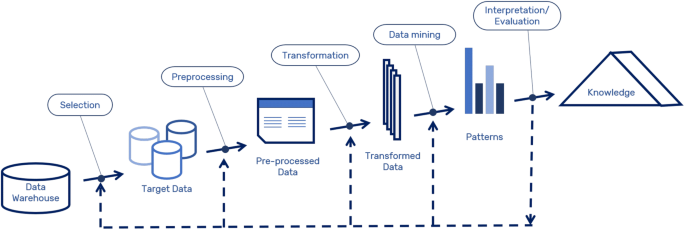
\includegraphics[width=12cm]{tcc_example/42979_2020_117_Fig3_HTML.png}
    \caption{KDD process model\cite{rotondo2020evolution}}
\end{figure}

O processo de KDD pode ser dividido em várias etapas\cite{marban2009data}, que são geralmente representadas pelo modelo CRISP-DM (CRoss-Industry Standard Process for Data Mining).

\begin{enumerate}
    \item \textbf{Entendimento dos dados}
    Aqui, é necessário explorar e analisar os dados disponíveis. Isso inclui a identificação das fontes de dados relevantes, a compreensão da estrutura dos dados, a avaliação da qualidade dos dados e a identificação de possíveis problemas ou limitações. 


 \item \textbf{Pré-processamento dos dados}
   Nesta etapa, os dados são preparados para a análise. Isso pode envolver a limpeza dos dados, a remoção de valores ausentes ou inconsistentes, a transformação dos dados em um formato adequado e a seleção das variáveis relevantes para a análise.
    
    \item \textbf{ransformação dos dados}
  qui, os dados são transformados em uma forma adequada para a aplicação de técnicas de mineração de dados. Isso pode incluir a normalização dos dados, a redução de dimensionalidade e a criação de novas variáveis ou características derivadas dos dados originais.

    \item \textbf{Mineração de dados}
  Nesta etapa, são aplicadas técnicas de mineração de dados para descobrir padrões, tendências ou relações nos dados. 

      \item \textbf{Avaliação dos resultados}
  s resultados da mineração de dados são avaliados para determinar sua relevância e utilidade. Isso pode envolver a análise estatística dos resultados, a validação cruzada, a comparação com critérios de desempenho ou a avaliação do impacto dos resultados nas metas de negócio. 



\end{enumerate}

E, por último, vem a interpretação e visualização dos dados. É neste ponto que entramos no âmago da mineração de processos. Após concluir toda a estruturação e preparação dos dados, aplicam-se algoritmos que geram os fluxos de processos. Nessa etapa, os resultados são apresentados de forma didática e de fácil compreensão para os usuários finais.\cite{marban2009data}


\section{Ciência de Processos}

A ciência de processos é uma área interdisciplinar que estuda processos - séries coerentes de mudanças que ocorrem em vários níveis e se desdobram ao longo do tempo - em múltiplos domínios \cite{vom2021process} físicos, químicos, biológicos ou outros que ocorrem em sistemas naturais ou artificiais. Este campo abrange uma variedade de disciplinas científicas e engenharia, com aplicações em diversas áreas, incluindo produção industrial, química, biologia, medicina, entre outros. A ciência de processos visa entender os mecanismos fundamentais que regem esses processos e, a partir desse entendimento, desenvolver métodos para otimizar ou controlar esses processos para atingir determinados objetivos.

A evolução da ciência de processos ao longo do tempo está fortemente ligada ao avanço da ciência e tecnologia em geral. Suas raízes podem ser rastreadas até os primeiros estudos em disciplinas como química, física e engenharia, que começaram a investigar os princípios básicos por trás de fenômenos naturais e técnicas de produção. No entanto, o termo "ciência de processos" ganhou popularidade mais recentemente, à medida que a compreensão da física e da química de sistemas complexos se tornou mais avançada.

Com o desenvolvimento da física moderna, química e engenharia, a ciência de processos se tornou cada vez mais interdisciplinar, integrando princípios de diferentes campos para entender e controlar processos em diversas escalas, desde o nível molecular até o macroscópico. Além disso, o avanço da tecnologia da informação e da computação tem desempenhado um papel significativo na evolução da ciência de processos, possibilitando simulações mais precisas e modelos preditivos mais complexos.

A ciência de processos também é valorizada porque busca criar conhecimento que tenha valor instrumental na solução de problemas do mundo real. Diante dos desafios globais enfrentados atualmente, essa área de pesquisa pode contribuir para o desenvolvimento de soluções eficazes e inovadoras, tanto na forma de organizar processos quanto na maneira de intervir neles.

Portanto, a ciência de processos é considerada um campo importante de pesquisa, pois proporciona uma compreensão aprofundada dos processos e oferece abordagens para projetar intervenções e moldá-las de acordo com nossas metas e objetivos.
 \cite{vom2021process}
 

\subsection{Framework da ciência de Processos 
}
\begin{figure}[h]
    \centering
    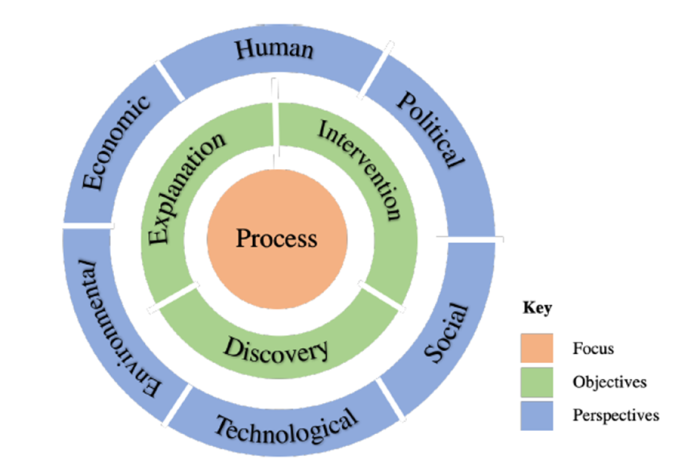
\includegraphics[width=12cm]{tcc_example/image-700x471.png}
    \caption{Framework da ciência de Processos \cite{vom2021process}}
\end{figure}

Para obter uma compreensão mais aprofundada dos princípios subjacentes à mineração de processos, o framework mencionado por \cite{vom2021process} oferece uma análise abrangente e perspicaz das ênfases e abordagens centrais desse campo em constante evolução. 

Enfoque: O cerne da mineração de processos gira em torno da análise dos processos.

Metas: A finalidade é a descoberta, explicação e intervenção nos processos.

Primeiramente, a etapa de descoberta enfoca a identificação das dinâmicas que constituem o fenômeno de interesse. As técnicas de mineração de processos desempenham um papel fundamental nessa fase, empregando dados de rastreamento digital para explorar uma ampla variedade de fenômenos, sejam eles de natureza organizacional ou natural.\cite{chia1999rhizomic}

Em seguida, a etapa de explicação busca compreender a dinâmica subjacente dos processos, explicando como e por que ocorrem e procurando identificar as relações de causa e efeito entre eles. Uma compreensão aprofundada dos processos permite realizar previsões sobre seus possíveis estados futuros.\cite{lazer2020computational}

Por fim, a intervenção tem como objetivo a modificação dos processos à medida que se desenrolam. Dessa forma, contribuímos de maneira mais eficaz para resolver problemas do mundo real.\cite{gaieck2020science}


\subsection{Principios Fundamentais da Ciência de Processos}

A mineração de processos é uma abordagem analítica que envolve a descoberta, monitoramento e melhoria de processos de negócios, utilizando técnicas de análise de dados para identificar padrões, tendências e insights a partir de dados de eventos registrados. Abaixo estão os passos comuns envolvidos no processo de mineração de processos


\begin{enumerate}
    \item \textbf{Colocar os processos no centro das atenções:}
    A Ciência de Processos se concentra em entender os processos - séries coerentes de mudanças que ocorrem em vários níveis e se desdobram ao longo do tempo. \cite{davenport2019process}


 \item \textbf{investigar os processos cientificamente:}
    A Ciência de Processos busca investigar os mecanismos e os impulsionadores que criam, desencadeiam, promovem ou retardam os processos, tanto naturais quanto feitos pelo homem\cite{davenport2019process}
    
    \item \textbf{Abraçar perspectivas de múltiplas disciplinas:}
  A Ciência de Processos é uma abordagem interdisciplinar, que integra contribuições de várias disciplinas para estabelecer uma compreensão abrangente dos processos e para projetar intervenções neles .\cite{davenport2019process}

    \item \textbf{Buscar impacto através da influência e mudança dos processos:}
   A Ciência de Processos tem como objetivo criar conhecimento que tenha valor instrumental na solução de problemas do mundo real e desenvolver soluções eficazes para desafios globais.\cite{davenport2019process}


\end{enumerate}

\section{Mineração de processos}

A mineração de processos, resultante da união da ciência de processos com a ciência de dados, é uma abordagem inovadora que visa analisar e aprimorar os processos organizacionais por meio da exploração de logs de eventos gerados por sistemas de informação.\cite{van2012process}
Ao combinar os conhecimentos técnicos e analíticos da ciência de processos com as habilidades de manipulação e interpretação de grandes conjuntos de dados da ciência de dados, a mineração de processos oferece insights valiosos para compreender, otimizar e automatizar os processos de negócios.

A análise e a melhoria de processos de negócios muitas vezes dependem da existência de modelos de processo precisos que retratam as características operacionais de uma organização. No entanto, a falta de modelos de processo completos e precisos é uma realidade em muitas organizações. Aqui é onde a mineração de processos entra em ação, utilizando técnicas e algoritmos avançados para descobrir e extrair automaticamente os modelos de processo subjacentes a partir dos registros de eventos.

Ao unir conceitos consolidados de administração, estatística e computação, a mineração de processos se torna uma ferramenta poderosa para a análise de dados orientada ao processo. Na indústria, o uso de ferramentas avançadas de mineração de processos pode impulsionar a eficiência operacional, aprimorar a qualidade do produto e serviço e fornecer uma vantagem competitiva significativa. Portanto, compreender os fundamentos da mineração de processos e estar ciente das ferramentas essenciais para sua implementação é crucial para aproveitar todo o potencial dessa abordagem inovadora.

\subsection{Motivação Principal:}

A motivação principal da mineração de processos é extrair conhecimento dos registros de eventos em ordem para descobrir, monitorar e melhorar processos reais.\cite{van2012process}

Essa compreensão detalhada dos desvios e exceções dos modelos normativos é vital para estabelecer uma abordagem adaptativa e flexível em relação aos processos organizacionais. Em vez de uma visão rígida e inflexível dos processos, a mineração de processos permite uma compreensão mais profunda das razões subjacentes às práticas operacionais, permitindo que as organizações respondam de maneira mais ágil e eficaz a mudanças e desafios em constante evolução.

Ao capturar esses desvios, a mineração de processos oferece insights valiosos sobre as práticas reais e identifica oportunidades para ajustes e melhorias contínuas nos modelos de processo. Isso cria uma base sólida para a adaptação dos processos normativos, garantindo que eles permaneçam alinhados com as práticas operacionais reais e promovam a eficiência e a eficácia organizacional.



\subsection{Principios da Mineração de Processos}

A mineração de processos é uma abordagem analítica que envolve a descoberta, monitoramento e melhoria de processos de negócios, utilizando técnicas de análise de dados para identificar padrões, tendências e insights a partir de dados de eventos registrados. Abaixo estão os passos comuns envolvidos no processo de mineração de processos\cite{van2012process}


\begin{enumerate}
    \item \textbf{Coleta de dados:} O primeiro passo é obter os dados de eventos relevantes para o processo que será analisado. Esses dados podem ser obtidos a partir de sistemas de informação, registros de atividades ou qualquer outra fonte que registre eventos relacionados ao processo.\cite{van2012process}

    \item \textbf{Pré-processamento dos dados:}  Os dados coletados podem precisar ser pré-processados para remover ruídos, tratar valores ausentes ou inconsistentes e garantir a qualidade dos dados. Isso pode envolver a limpeza dos dados, a padronização de formatos e a normalização de valores.\cite{van2012process}
    
    \item \textbf{Descoberta do modelo de processo: } Nesta etapa, algoritmos de descoberta de processos são aplicados aos dados para identificar padrões e relações entre as atividades do processo. Isso resulta na criação de um modelo de processo que representa a sequência de atividades e as dependências entre elas.\cite{van2012process}

      \item \textbf{Análise do modelo de processo: } O modelo de processo descoberto é analisado para identificar gargalos, desvios, padrões de comportamento e outras informações relevantes. Isso pode envolver a identificação de atividades que consomem mais tempo, a detecção de desvios em relação ao modelo esperado e a identificação de possíveis melhorias no processo.\cite{van2012process}

       \item \textbf{Conformidade do processo:} conformidade do processo é verificada comparando o modelo de processo descoberto com as regras e restrições definidas para o processo. Isso permite identificar desvios e inconsistências entre o modelo e a execução real do processo.\cite{van2012process}


        \item \textbf{Melhoria do processo:} m base nas análises realizadas, são propostas melhorias para o processo, como otimização de atividades, redefinição de fluxos de trabalho ou realocação de recursos. Essas melhorias visam aumentar a eficiência, reduzir custos e melhorar a qualidade do processo.\cite{van2012process}

          \item \textbf{Descoberta do modelo de processo: } Nesta etapa, algoritmos de descoberta de processos são aplicados aos dados para identificar padrões e relações entre as atividades do processo. Isso resulta na criação de um modelo de processo que representa a sequência de atividades e as dependências entre elas.\cite{van2012process}

          A mineração de processos é uma abordagem que se concentra na ideia de primeiro "descobrir" padrões e estruturas significativos em conjuntos de dados de registro de eventos, para então, posteriormente, utilizar essas descobertas para construir modelos analíticos e preditivos que possam fornecer insights valiosos sobre os processos subjacentes.\cite{greyling2017application}. Os modelos contruídos dessa maneira são capazes de transmitir as atividades do mundo real pertencentes a um processo

          Para realizar a mineração de processos e em seguida a descoberta do modelo de processos os seguintes atributos de dados são necessários: 




\end{enumerate}



\subsection{Log de Processos}

Para realizar a mineração de processos e em seguida a descoberta do modelo de processos os seguintes atributos de dados\cite{greyling2017application} são necessários:  

\vspace{1cm}


\begin{table}[ht]
\centering
\begin{tabularx}{0.8\textwidth} { 
  | >{\raggedright\arraybackslash}X 
  | >{\centering\arraybackslash}X 
  | >{\raggedleft\arraybackslash}X | }
 \hline
 Identificação do evento & Esses IDs são atribuídos às atividades do processo. IDs podem ser gerados à medida que as atividades ocorrem ou ter um valor fixo para tipos de eventos  \\
 \hline
 Timestamp  & Os timestamps são atribuídos no instante em que o status de um evento é acionado    \\
\hline
 Atividade  & Uma descrição do evento    \\
\hline
Recurso  & Refere-se à pessoa ou entidade responsável pela realização do evento   \\
\hline
Identificação do caso  & Esses IDs são atribuídos de acordo com a instância de processo (caso) à qual as atividades pertencem   \\
\hline
\end{tabularx}
\caption{Atributos de dados.\cite{greyling2017application}}
\label{tab:minhatabela}
\end{table}



\vspace{1cm}

Com esses atributos citados na tabela acima, as atividades pedem ser modeladas a partir de diferentes perspectivas\cite{greyling2017application}, sendo:

\begin{enumerate}
    \item \textbf{Uma perspectiva de fluxo de controle:}que ilustra as definições dos processos e a ordem das atividades.
    
    \item \textbf{Uma perspectiva de recursos:} que dá uma visão organizacional da estrutura do processo e do atores envolvidos
    
    \item \textbf{Uma perspectiva de dados:} Ilustrando a informação gerada no processo

     \item \textbf{Uma perspectiva de tarefa:} Que é indicativa da função organizacional envolvida no processo (ou seja, as operações)

      \item \textbf{perspectiva operacional} lustrando a aplicação do processo e as ações
\end{enumerate}

 é uma ferramenta essencial para a análise e melhoria de processos. Ele fornece dados concretos sobre como os processos são executados na prática, permitindo a identificação de problemas e oportunidades de melhoria. Como afirmado no artigo, "A mineração de processos é uma técnica valiosa que deve fazer parte do conjunto de ferramentas de melhoria de qualquer Gestor"\cite{greyling2017application}.


\subsection{Revisão de Algoritmos}

Antes de construir um modelo a partir de um registro de eventos, é essencial realizar a extração e organização dos dados. Dentro do campo da mineração de processos, existem vários tipos de algoritmos que são aplicados para extrair os dados de acordo com determinadas regras, dependendo do comportamento específico que se deseja observar. Cada um desses algoritmos apresenta suas próprias vantagens e desvantagens distintas. Se observarmos de forma holística, podemos identificar três categorias principais de algoritmos utilizados na mineração de Processos.

\subsubsection{Algoritmos determinísticos}

    o lidar com modelos determinísticos, todos os dados necessários para a obtenção do resultado na mineração de processos são conhecidos previamente. Uma das propriedades mais notáveis dos modelos determinísticos é a estabilidade da saída do processo de mineração em relação às variáveis de entrada fornecidas no registro de eventos. Isso implica que o modelo criado durante o procedimento de mineração de processos é consistentemente reproduzível. Além disso, é possível evidenciar que os algoritmos determinísticos tendem a ter um desempenho mais ágil quando comparados a outros tipos de algoritmos \cite{colacco2011survey}. 

    \subsubsection{Algoritmos heurísticos}

    Algoritmos heurísticos são frequentemente empregados quando uma abordagem algorítmica predefinida não consegue encontrar uma solução ótima. Em tais cenários, é crucial adotar uma abordagem que busque alcançar uma solução satisfatória, mesmo que não seja globalmente ideal, por meio de tentativa e erro \cite{winston2004operations}. No contexto da mineração de processos, os algoritmos determinísticos servem como base, complementados por princípios de Pareto, indicando a importância da frequência, a fim de descartar caminhos ou eventos que apenas resultam em uma complexidade desnecessária.
    
\subsubsection{Algoritmos genéticos} 

    Os algoritmos genéticos têm sua origem nos princípios fundamentais que regem a seleção natural na teoria evolucionária [16]. Ao adotar os algoritmos genéticos, o processo de encontrar uma solução para um problema começa a partir de um ponto inicial arbitrária e, progressivamente, busca-se aprimorar essa solução, descartando aquelas consideradas inferiores. Essa busca é conduzida pela combinação de características derivadas de soluções anteriores, bem como pela introdução de variações aleatórias, permitindo a exploração de novas possibilidades e caminhos.

O procedimento dos algoritmos genéticos segue um processo estruturado em cinco etapas bem definidas\cite{greyling2017application}, representando uma abordagem abrangente e sistematizada para enfrentar problemas complexos de forma eficaz e eficiente.

\begin{enumerate}
    \item \textbf{Gerar soluções aleatórias e avaliar a adequação do modelo gerado}
    
    \item \textbf{Cruzamento: Gerar descendentes (novas soluções) usando a melhor solução na etapa anterior}
    
    \item \textbf{Mutação}  Inserir variações aleatórias no espaço de solução
    
     \item \textbf{Atribuição de adequação}Atribuir um valor de adequação às soluções com base no resultado

      \item \textbf{Seleção} Selecionar as melhores soluções com base na adequação e usá-las para a próxima etapa de cruzamento até que o critério seja satisfeito.

      \end{enumerate}

Segue a logica onde modelos de processo são gerados aleatoriamente e em seguida, reduzidos iterativamente para encontrar soluções mais satisfatorias por meio das etapas de (mutação e cruzamento). Deve-se entender que os modelos de processo iniciais não são uma representação do registro de eventos.

Dentro de cada estudo de mineração de processos é fundamental identificar as necessidades do estudo. isso permite a seleção adequada do algoritmo e garante que o modelo não esteja subajustado. 

São utilizados Criterios\cite{greyling2017application} que vão estar citados na tabela abaixo que exibem alguns dados gerados ondem podemos enxergar o desempenho do algoritmo aplicado sendo:

\begin{table}[ht]
\centering
\begin{tabularx}{0.8\textwidth} { 
  | >{\raggedright\arraybackslash}X 
  | >{\centering\arraybackslash}X 
  | >{\raggedleft\arraybackslash}X | }
 \hline
 Precision &  modelo não permite caminhos que diferem da realidade \\
 \hline
 Fitness  & A capacidade de reproduzir exatamente o que aconteceu no registro de eventos    \\
\hline
 Simplicity  & Reduzir a complexidade do modelo eliminando caminhos indesejados    \\
\hline
Generalisability  &  O modelo não é exclusivo para um determinado registro de eventos e pode ser usado para fazer generalizações sobre outros processos.   \\
\hline
\end{tabularx}
\caption{Criterios de avaliação do modelo. \cite{greyling2017application}}
\label{tab:minhatabela}
\end{table}


\vspace{1cm}

Dificilmente será possivel atender todos esses criterios ao mesmo tempo, a importancia de cada criterio precisa der avaliada em determinadas ocasiões.


\subsection{Modelos de processos de negócios}

\subsection{Redes de petri}

A Rede de Petri é uma ferramenta gráfica e matemática que se adapta facilmente a uma ampla variedade de aplicações em que conceitos de eventos e evoluções simultâneas são fundamentais.\cite{cardoso1997redes}

"Esta teoria é muito jovem, pois nasceu da tese, intitulada Comunicação com autômatos,
defendida por Carl Adam Petri em 1962 na Universidade de Darmstadt, Alemanha. Carl
Adam Petri, nascido em 1926 em Leipzig, e professor na Universidade de Bonn. Anatol
W. Holt foi seduzido por este trabalho e sob sua impulsão um grupo de pesquisadores
do Massachussetts Institute of Technology-MIT, Estados Unidos, lançaa as bases, entre
1968 e 1976, do que se tornou as redes de Petri. Entre estes pioneiros destacam-se F.
Commoner e M. Hack."\cite{cardoso1997redes}

Dentre as inúmeras aplicações, pode-se mencionar: avaliação de desempenho, análise e verificação formal em sistemas discretos, protocolos de comunicação, controle de oficinas de fabricação, concepção de software em tempo real e/ou distribuído, sistemas de informação (para organização de empresas), sistemas de transporte, logística, gerenciamento de banco de dados, interface homem-máquina e multimídia.

As Redes de Petri podem ser utilizadas na mineração de processos como uma representação gráfica poderosa para modelar e analisar sistemas dinâmicos. Elas ajudam a visualizar e entender o fluxo de trabalho em um processo e podem ser empregadas de diversas maneiras nesse contexto



\begin{figure}[h]
    \centering
    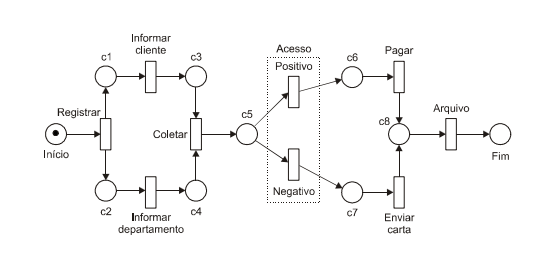
\includegraphics[width=12cm]{tcc_example/rede_petri.png}
    \caption{Rede Petri\cite{cardoso1997redes}}
\end{figure}

\subsection{BPMN}

O BPMN (Business Process Model and Notation) é um padrão para representar processos de negócios de forma gráfica. Ele gera uma imagem visual que mostra as atividades, eventos, gateways e fluxos de um processo. O BPMN é amplamente utilizado em várias organizações e setores devido à sua capacidade de fornecer uma representação clara e compreensível dos processos.\cite{chinosi2012bpmn}

Em comparação, os modelos de Petri e as árvores de processos têm uma abordagem mais formal e matemática para representar os processos. Eles são mais adequados para análises detalhadas e simulações precisas, mas podem ser menos acessíveis para usuários de negócios que não possuem conhecimentos técnicos avançados.

\begin{figure}[h]
    \centering
    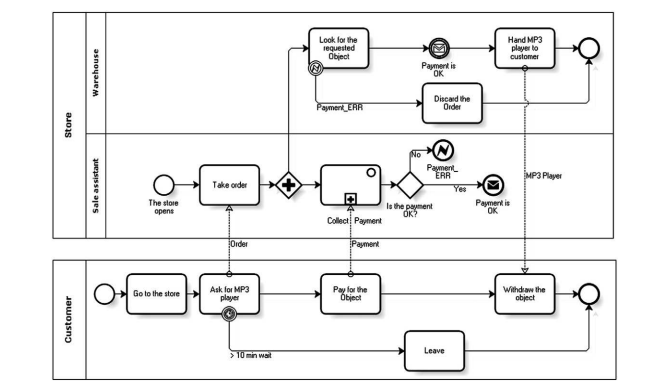
\includegraphics[width=12cm]{tcc_example/bpmn.png}
    \caption{Rede BPMN\cite{chinosi2012bpmn}}
\end{figure}

ela é simples de ser interpretada, o circulo verde representa o inicio da cadeia de processos, cada um desses retangulos representa uma etapa, os losangulos com um X dentro representam um ponto de desvio ou decisão, e o circulo laranja representa o final de toda essa cadeia.

Em resumo, o BPMN é uma notação gráfica amplamente utilizada para representar processos de negócios. Ele oferece uma representação visual clara e compreensível, mas pode ser complexo devido à sua variedade de elementos e regras de modelagem. Em comparação com os modelos de Petri e árvores de processos, o BPMN é mais acessível para usuários de negócios, mas pode ser menos adequado para análises detalhadas e simulações precisas.

\subsection{Process Tree}

A Árvore de Processos, também conhecida como Process Tree, é um modelo estocástico utilizado no campo da mineração de processos. Ela constitui uma representação gráfica das diversas etapas e decisões que compõem um processo, viabilizando a análise e a compreensão do fluxo de trabalho dentro de uma organização.\cite{erdfelder2009multinomial}

O funcionamento da Árvore de Processos envolve a criação de um modelo probabilístico que descreve as possíveis sequências de eventos em um processo. Cada evento é representado por um nó na árvore, enquanto as transições entre os eventos são simbolizadas por ramos. Adicionalmente, é possível designar probabilidades às transições, indicando a probabilidade de uma determinada transição ocorrer em comparação com outras possíveis transições.

Na prática da mineração de processos, a Árvore de Processos é empregada para analisar e extrair informações relevantes acerca do comportamento dos processos em uma organização. Ela pode ser aplicada em diversas áreas, como logística, saúde, manufatura, entre outras, a fim de identificar gargalos, reconhecer padrões de comportamento, otimizar processos e embasar decisões com base em dados.\cite{erdfelder2009multinomial}

Em síntese, a Árvore de Processos representa uma ferramenta poderosa na mineração de processos, permitindo uma análise detalhada e probabilística do fluxo de trabalho em uma organização, e contribuindo para a identificação de oportunidades de aprimoramento e para a tomada de decisões fundamentadas em dados.

\begin{figure}[h]
    \centering
    
\includegraphics[width=12cm]{tcc_example/process_tree_running_example.png}
    \caption{Process Tree exemplo }
\end{figure}

O modelo da árvore de processos é construido  de cima para baixo. O primeiro círculo, que é a 'raiz' da árvore de processos, é representado por um símbolo '->'. Isso indica que, ao seguir para baixo, o processo descrito pelo modelo executa os 'filhos' da raiz da esquerda para a direita. Dessa forma, a primeira “solicitação de registro” é executada, seguida pelo nó do círculo com o símbolo '', e, por fim, seguida pelo nó com o símbolo 'X'. O nó com '' representa 'comportamento repetido', ou seja, a possibilidade de repetir o comportamento. Ao descer mais na árvore, a 'subárvore' mais à esquerda do operador '' é sempre executada, enquanto o filho mais à direita (neste caso, “solicitação de reinicialização”) aciona uma repetição da execução do filho mais à esquerda. É importante notar que isso está de acordo com os modelos de processo previamente discutidos, ou seja, a atividade “reiniciar solicitação” nos permite repetir o comportamento em relação aos exames e à verificação do ticket. Ao continuar descendo na subárvore do operador '', encontramos novamente um nó '->'. Portanto, seu filho mais à esquerda é executado primeiro, seguido por seu filho mais à direita (“decidir”). O filho mais à esquerda do nó '->' possui um símbolo '+', que representa comportamento simultâneo; assim, seus filhos podem ser executados simultaneamente ou em qualquer ordem. O filho mais à esquerda é a atividade “verificar ticket”, enquanto o filho mais à direita é um nó com o símbolo 'X' (semelhante ao filho mais à direita da raiz da árvore). Isso representa uma escolha exclusiva, ou seja, uma das atividades é executada (ou “examinar casualmente” ou “examinar minuciosamente”).\cite{erdfelder2009multinomial}



Em resumo, o BPMN é uma notação gráfica amplamente utilizada para representar processos de negócios. Ele oferece uma representação visual clara e compreensível, mas pode ser complexo devido à sua variedade de elementos e regras de modelagem. Em comparação com os modelos de Petri e árvores de processos, o BPMN é mais acessível para usuários de negócios, mas pode ser menos adequado para análises detalhadas e simulações precisas.

\chapter{Métodos}

A análise de processos é crucial para entender e otimizar a eficiência operacional e a eficácia dos processos em uma organização. Cada um dos algoritmos que você empregou oferece abordagens distintas para a descoberta de modelos de processo a partir dos dados de logs, o que pode ajudar a identificar padrões, gargalos e ineficiências nos processos organizacionais. 

Vamos empregar diversas ferramentas no desenvolvimento do nosso algoritmo. Optaremos pela linguagem de programação Python, aproveitando a biblioteca pm4py para aplicar algoritmos de leitura e descoberta de processos de forma eficiente.

\subsection{Phyton}

Python se destaca como uma linguagem de programação poderosa e elegante, reconhecida por sua legibilidade e compreensibilidade. Sua versatilidade a torna aplicável a uma ampla variedade de cenários, destacando-se especialmente na análise de dados. A simplicidade e clareza de sua sintaxe facilitam a redação de código, tornando-o acessível a programadores de diversos níveis.\cite{python2021python}

\subsection{Pm4py}

PM4Py é uma biblioteca em Python que fornece uma ampla variedade de ferramentas para process mining, ou seja, a análise de dados de eventos para entender e melhorar processos operacionais. A biblioteca oferece recursos como descoberta de processos, verificação de conformidade e aprimoramento de processos, e suporta diferentes formatos de dados. PM4Py é uma ferramenta essencial para pesquisadores e profissionais da área, sendo amplamente adotada na academia, indústria e comunidade de código aberto. Ela tem sido usada no desenvolvimento de várias ferramentas de software de process mining.\cite{berti2023pm4py}



\subsection{Base de dados}

Esses dados constituem a base para testar algoritmos de process mining, focando em um processo de solicitação de empréstimo de uma instituição financeira na Holanda. As informações abrangem todas as inscrições feitas por meio do sistema online durante o ano de 2016 e os eventos subsequentes até 1º de fevereiro de 2017, às 15h11. O identificador DOI para esse conjunto de dados é 10.4121/uuid:3926db30-f712-4394-aebc-75976070e91f, vinculando os dados à mesma empresa responsável pelo processo.

É importante destacar que houve uma alteração no sistema que suporta o processo ao longo do tempo. Em particular, o sistema agora permite a apresentação de várias ofertas para uma única aplicação. Essas ofertas podem ser rastreadas por meio de seus IDs no registro.

\subsection{Aplicação dos algoritmos}

\subsubsection{Alpha Miner}

O Alpha Miner é um algoritmo amplamente utilizado no campo da mineração de processos. Ele é capaz de descobrir modelos de processos a partir de logs de eventos. Uma das principais vantagens do Alpha Miner é sua capacidade de lidar com a concorrência em processos, o que o torna adequado para analisar atividades de aprendizado online que podem ocorrer simultaneamente.\cite{nafasa2019implementation}

O Alpha Miner Possui uma capacidade  de construir automaticamente modelos de processos na forma de Redes de Petri, sem a necessidade de conhecimento adicional. Isso torna o algoritmo fácil de usar e acessível para usuários sem experiência em mineração de processos.

No entanto, o Alpha Miner também apresenta algumas desvantagens. Por exemplo, ele pode ter dificuldades em lidar com loops curtos em dados de log, o que pode levar a resultados imprecisos ou incompletos. Além disso, o Alpha Miner pode não ser adequado para todos os tipos de processos, especialmente aqueles com estruturas complexas ou padrões de fluxo de controle não lineares.\cite{nafasa2019implementation}

Em termos de funcionamento, o Alpha Miner analisa os logs de eventos para identificar padrões de ocorrência de atividades. Com base nesses padrões, ele constrói um modelo de processo que representa a sequência de atividades e as relações de dependência entre elas. O algoritmo utiliza técnicas de análise de grafos e heurísticas para identificar as transições e lugares do modelo de processo.


Em resumo, o Alpha Miner é um algoritmo poderoso para a descoberta de modelos de processos a partir de logs de eventos. Embora tenha suas vantagens e desvantagens, ele desempenha um papel importante na análise de atividades de aprendizado online e na melhoria da qualidade do ensino.

\subsubsection{Inductive Miner}

O Inductive Miner é um algoritmo proposto para a descoberta de modelos em dados educacionais. Ele difere de outros algoritmos, como o Alpha Miner, o Heuristic Miner e o Evolutionary Tree Miner, por sua abordagem indutiva.\cite{bogarin2018discovering}

Uma das principais vantagens do Inductive Miner é sua capacidade de produzir resultados superiores em relação a outros algoritmos em termos de ajuste (fitness).

\subsubsection{Heuristics Miner}

O Heuristics Miner é um algoritmo de mineração de processos que é usado para descobrir modelos de processos a partir de registros de eventos. Ele conta várias frequências para identificar as relações de dependência entre as atividades representadas nos logs. O algoritmo utiliza a relação "a >W b", que indica que a atividade "b" segue diretamente a atividade "a" em uma determinada sequência de eventos. O Heuristics Miner utiliza diferentes métricas e fórmulas para construir um modelo de processo com base nessas relações de dependência. Ele pode ser adaptado para lidar com fluxos contínuos de eventos, permitindo a descoberta de modelos de processo em tempo real.\cite{burattin2012heuristics}


\subsection{O algoritmo}

O algoritmo tem o objetivo de realizar a descoberta de redes de Petri utilizando três algoritmos diferentes (Alpha Miner, Inductive Miner, Heuristics Miner) a partir de um arquivo de log no formato XES. Após a descoberta, ele avalia o desempenho dessas redes utilizando métricas como fitness, precisão e generalização. Finalmente, o código cria gráficos de barras para comparar essas métricas entre os algoritmos.

possui alguns passos principais 

\begin{enumerate}
    \item \textbf{Leitura do Arquivo de Log:} um arquivo de log no formato XES é lido, fornecendo os dados de eventos necessários para a análise.
    
        \item \textbf {Descoberta de Redes de Petri:} Utiliza três algoritmos de descoberta de redes de Petri para obter modelos de processo a partir do log de eventos.
    
    \item \textbf{Avaliação das Redes de Petri Descobertas:} Utiliza três algoritmos de descoberta de redes de Petri, para obter modelos de processo a partir do log de eventos.
    

     \item \textbf{Preparação dos Dados para Visualização:} Organiza os resultados da avaliação em listas para facilitar a criação dos gráficos de barras.

      \item \textbf{Visualização dos Resultados:} Cria gráficos de barras para comparar as métricas (fitness, precisão, generalização) entre os algoritmos. Cada métrica tem seu próprio gráfico.
\end{enumerate}

 A criação de gráficos de barras facilita a comparação visual das métricas entre os algoritmos, permitindo uma análise rápida do desempenho relativo de cada abordagem na descoberta de redes de Petri.

\subsubsection{Aplicação Alpha Miner }
Começando com o Alpha Miner, este algoritmo é conhecido por sua simplicidade e eficácia na descoberta de redes de Petri diretamente dos registros de eventos. Ele é capaz de identificar relações causais entre atividades e construir um modelo de processo básico, sem exigir muitos parâmetros de entrada. No entanto, devido à sua abordagem simplista, pode ter dificuldades em capturar nuances mais complexas presentes nos dados do log de eventos.

\begin{figure}[h]
    \centering
    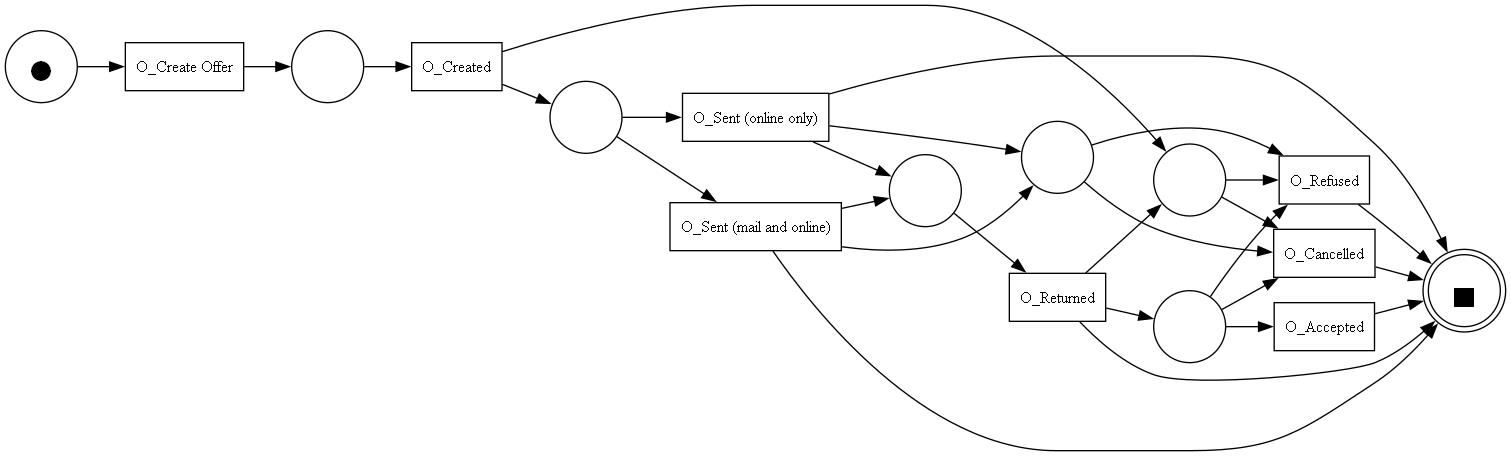
\includegraphics[width=12cm]{tcc_example/Alpha_miner.jpg}
    \caption{Rede Petri Algoritmo Alpha Miner}
\end{figure}

Resultados do Algoritmo Alpha Miner

\begin{enumerate}
    \item \textbf{Fitness:} Observou-se que o modelo gerado pelo Alpha Miner possui um fitness global de aproximadamente (78.98). Isto significa que o modelo representa adequadamente os padrões observados no log de eventos, embora haja espaço para melhorias.
    
        \item \textbf {Precisão:} O Alpha Miner alcançou uma precisão perfeita de 100 por cento. Isso sugere que o modelo criado é totalmente preciso em reproduzir as variantes do log de eventos.
    
    \item \textbf{Generalização:} A generalização do modelo Alpha Miner foi de aproximadamente 99.09 por cento. Este valor indica que o modelo consegue generalizar bem os comportamentos do log de eventos.
    
\end{enumerate}

\subsubsection{Aplicação Inductive Miner }
Por outro lado, o Inductive Miner é conhecido por sua capacidade de lidar com complexidades e variações nos dados do log de eventos. Ele constrói modelos de processo mais robustos, levando em consideração diferentes possibilidades e variações nos caminhos de processo. Ao fazer isso, é capaz de capturar melhor as nuances dos processos reais, o que o torna uma opção atraente ao lidar com dados mais complexos e variados.

\begin{figure}[h]
    \centering
    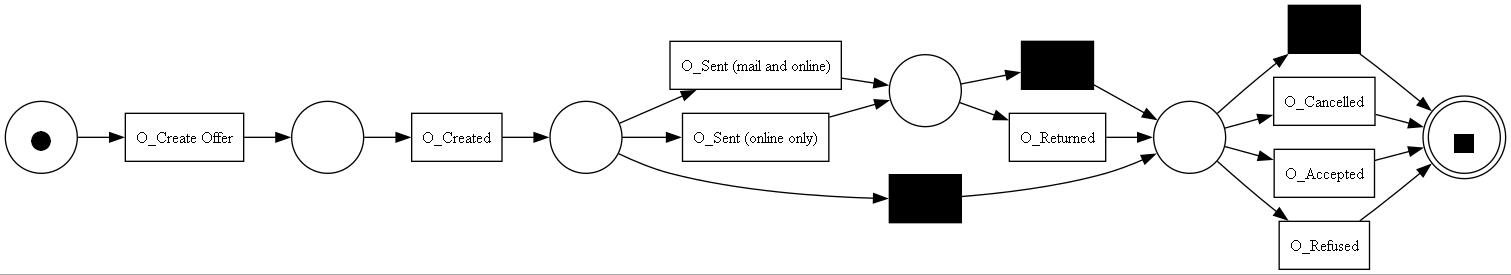
\includegraphics[width=12cm]{tcc_example/Indutivo_miner.jpg}
    \caption{Rede Petri Algoritmo Inductive Miner}
\end{figure}

Resultados do Algoritmo Inductive Miner

\begin{enumerate}
    \item \textbf{Fitness:} O modelo do Inductive Miner atingiu um fitness global de 100 por cento, indicando uma correspondência perfeita com os padrões observados no log de eventos.
    
        \item \textbf {Precisão:} A precisão foi de aproximadamente 87.70 por cento, sugerindo que, embora a maioria das variantes seja reproduzida corretamente, há algumas exceções.
    
    \item \textbf{Generalização:} A generalização do Inductive Miner foi de cerca de 98.33 por cento, indicando uma capacidade sólida de representar comportamentos gerais.
    
\end{enumerate}

\subsubsection{Aplicação Heuristics Miner }
O Heuristics Miner, por sua vez, é um compromisso entre os dois. Ele se destaca na descoberta de modelos de processo a partir de logs de eventos que podem conter uma quantidade considerável de ruído. Isso o torna particularmente útil em cenários onde os dados de log podem ser incompletos ou imprecisos. O Heuristics Miner utiliza técnicas heurísticas para inferir relações de precedência entre atividades e, assim, construir um modelo de processo que leve em consideração essas heurísticas.

\begin{figure}[h]
    \centering
    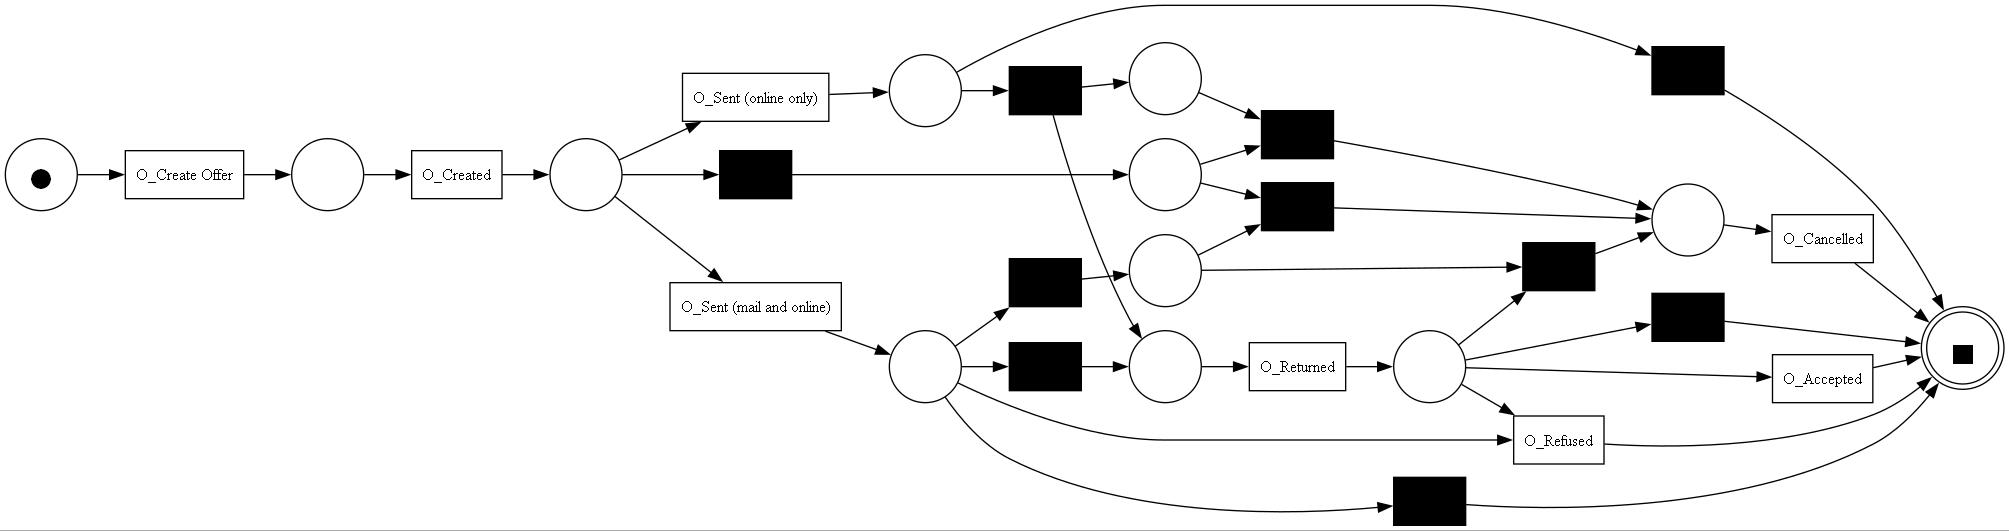
\includegraphics[width=12cm]{tcc_example/Heuristics_miner.jpg}
    \caption{Rede Petri Algoritmo Heuristics Miner}
\end{figure}

Resultados do Algoritmo Heuristics Miner

\begin{enumerate}
    \item \textbf{Fitness:} O modelo gerado pelo Heuristics Miner apresentou um fitness global de cerca de 91.37 por cento. Embora não seja perfeito, ainda reflete uma representação razoavelmente boa do log de eventos.
    
        \item \textbf {Precisão:} Assim como o Alpha Miner, o Heuristics Miner alcançou uma precisão de 100 por cento, indicando que reproduz corretamente todas as variantes do log de eventos.
    
    \item \textbf{Generalização:} A generalização do Heuristics Miner foi a mais baixa entre os algoritmos, com aproximadamente 79.89 por cento. Isso sugere que o modelo pode ter dificuldade em generalizar além dos padrões específicos do log de eventos.

    
\end{enumerate}



\chapter{Resultados} 

Os resultados da aplicação dos algoritmos de descoberta de redes de Petri, aliados à avaliação rigorosa das métricas de fitness, precisão e generalização, oferecem uma visão multifacetada e criteriosa sobre o desempenho dessas abordagens em relação ao conjunto de dados em questão.

\begin{figure}[h]
    \centering
    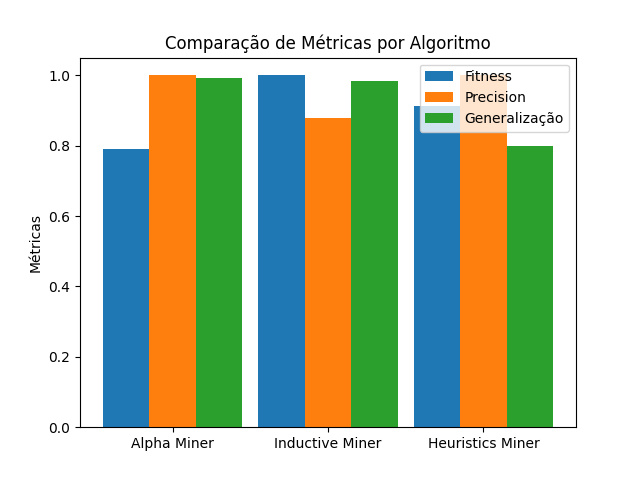
\includegraphics[width=12cm]{tcc_example/Figure_1.png}
    \caption{Resultados Comparatorios}
\end{figure}

Alpha Miner:

O Alpha Miner revelou-se um construtor sólido de modelos de processo, alcançando uma generalização notável de aproximadamente 99.09 por cento. Sua precisão perfeita indica uma fidelidade consistente com as variantes do log, apesar de um fitness global de 78.98 por cento, sugerindo espaço para aprimoramentos na correspondência global. Este algoritmo se destaca pela capacidade de representar eficazmente padrões gerais e comportamentos observados.
Inductive Miner:

O Inductive Miner demonstrou excelência na captura precisa dos eventos do log, atingindo um fitness global de 100 por cento. A precisão de 87.70 por cento destaca sua habilidade de reproduzir fielmente a maioria das variantes, enquanto a generalização de 98.33 por cento sublinha sua capacidade de abstrair padrões mais amplos. Este algoritmo se mostra particularmente robusto para cenários onde uma correspondência exata é essencial.
Heuristics Miner:

O Heuristics Miner, embora tenha evidenciado uma precisão perfeita de 100 por cento, apresentou uma generalização mais modesta de 79.89 por cento. Este resultado sugere uma sensibilidade a detalhes específicos do log, indicando que sua força reside na reprodução precisa de variantes específicas. A escolha deste algoritmo deve ser cuidadosamente ponderada, priorizando a fidelidade à reprodução das variantes observadas.

 A análise abrangente dos resultados obtidos através da aplicação dos algoritmos de descoberta de redes de Petri - Alpha Miner, Inductive Miner e Heuristics Miner - proporcionou uma compreensão detalhada de suas respectivas capacidades e nuances no contexto do nosso conjunto de dados. Cada algoritmo revelou aspectos distintos, desde a robustez na generalização até a precisão notável na reprodução de variantes específicas.

Diante dessas observações, reconhecemos que a busca contínua pela otimização dessas métricas fundamentais - fitness, precisão e generalização - pode ser um próximo passo crucial em nosso processo analítico. Para isso, propomos a aplicação de algoritmos genéticos, uma abordagem que tem mostrado grande promessa na busca por soluções eficientes e melhorias substanciais em diversos domínios.

A introdução de algoritmos genéticos no contexto da descoberta de redes de Petri permitirá a exploração sistemática do espaço de soluções, visando não apenas aprimorar as métricas já avaliadas, mas também descobrir novas abordagens que possam potencialmente elevar o desempenho global dos modelos gerados. Este enfoque estratégico alinha-se com a busca incessante por inovação e aprimoramento contínuo em nossas análises de processos.

Nesse cenário, o objetivo é não apenas selecionar o algoritmo de descoberta mais adequado para o conjunto de dados atual, mas também evoluir constantemente, adaptando-se a nuances e desafios específicos que possam surgir. Ao incorporar algoritmos genéticos, buscamos não somente atingir novos patamares de performance, mas também proporcionar uma resposta dinâmica e adaptativa às complexidades inerentes aos processos analisados.

Em suma, esta conclusão não é apenas um ponto final na análise atual, mas um ponto de partida para uma abordagem mais avançada e estratégica. Ao integrar algoritmos genéticos em nossos esforços, aspiramos aprimorar significativamente nossos modelos de processo, oferecendo resultados mais robustos e eficazes. Este movimento reflete nosso compromisso contínuo com a excelência analítica e a busca incessante por soluções inovadoras.



\backmatter 
\singlespacing   
% ----------------------------------------------------------------------------------------------------- %
\bibliography{tcc_exemplo}

\appendix
\onehalfspacing

\end{document}
